\section{INTRODUCTION}

  \begin{figure}
  \centering
  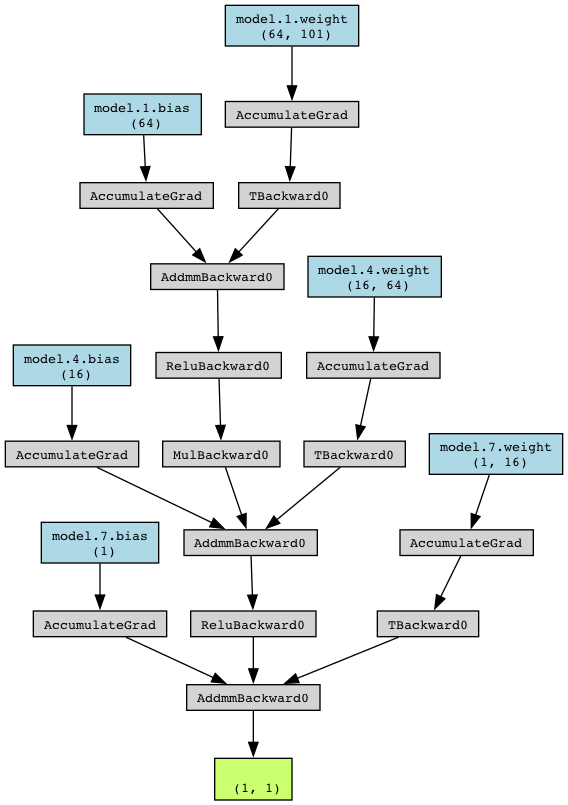
\includegraphics[width=3.5in]{viz.png}
  \caption{The neural network.}
  \label{fig:thennet}
  \end{figure}


  Fractional calculus and fractional order dynamics are increasingly important
  in modern engineered systems. Unlike integer order derivatives, fractional
  order derivatives, and hence the dynamics that depend on them, are
  \emph{nonlocal}. As such, many modern, large scale engineered systems may
  exhibit fractional order dynamics and responses because interactions among
  various components in the system may be significantly displaced in time or
  space. In instances where significant fractional order dynamics are present,
  control algorithms which directly address the fractional nature of the system
  may be superior.  Therefore, tools to readily identify if significant
  fractional order dynamics are present are needed.

  There is a vast literature on fractional calculus. Some textbooks include
  \cite{fracbook,fracbook2,oustaloup}.  Fractional-order control is considered
  in many topical areas, but particularly relevant to this paper is fractional
  order controls, such as in \cite{fraccontrol,YQChenAcc}. An excellent review
  article illustrating the very broad range of applications of fractional
  calculus and control in science and engineering is \cite{SUN2018213}.


  Our main interest are identifying cases where fractional order models may
  provide useful ``reduced order'' models for large scale systems
  \cite{goodwinemed2023,goodwinemmar2023} and for exact models for many large
  scale systems
  \cite{Goodwine2014Modeling,Leyden2016Using,Leyden2019Large,bg:xnids2022,bg:xninonlinear2020}.
  A fractional order system is arguably infinite order, but a fractional order
  representation is more concise than, for example, an extremely high order
  system like those considered in the preceding references.  While this paper
  does not build upon it, our closest publication to this would be
  \cite{bg:chenSII2022} where we created a symmetric neural network with a
  sequential set of identical layers. When it was trained on first derivatives
  of functions, the middle layer could represent the half derivative. 
 
 There are many different definitions of the fractional derivative. As will be
 outlined in the next section, a common feature of these is replacing factorial
 functions appearing in many integer-order representations of the derivative
 with gamma functions. The Riemann-Liouville, Caputo and the Gr\"unwald-Letnikov
 definitions are perhaps the most common examples of fractional derivative
 definitions, and the reader is referred to the references
 \cite{Machado20111140,4609961,series/lnee/Ortigueira11,das2011functional} for
 descriptions and definitions of each. Because of the python library we utilize
 for this paper, the definition used herein is the Caputo fractional derivative. 

 Machine learning in general and neural networks in particular have a long
 history. One of the earliest works related to the feed forward neural network,
 the type used in this paper, is from 1960 by Rosenblatt \cite{Rosenblatt1960}.
 In the 1970s, advanced in training by the back propagation method were
 developed \cite{linnainmaa1} and were further advanced in the 1980s
 \cite{werbos}.  Additionally in the 1980s theoretical advances such as the
 universal approximation theorem \cite{hornik1989multilayer} were developed.
 These practical advances buttressed with theoretical support helped advance the
 cause for usefulness of artificial neural networks. Of course, the confluence
 of ubiquitous data and advanced in computer processing power enabled many
 applications in the beginning of the 21st century has resulted in the rapid
 deployment throughout many aspects of modern life. 

 Because robotics and control systems are at the interface of computational
 intelligence and the physical world, there have been many applications of
 machine learning and neural networks in this realm. A comprehensive outline of
 the literature is not possible in a paper of this type. Several recent survey
 papers include \cite{semeraro,9199280,bai} highlighting a long list of
 application areas such as assembly and object handling in manufacturing, human
 robot interaction, object recognition and other vision applications, locomotion
 and path planning, transfer learning, localization, grasp detection, motion
 planning, whole body planning, sensor fusion, and many others.
 

 The rest of this paper is organized as follows. Section~\ref{sec:fractional}
 provides a limited introduction to fractional calculus, including the concepts
 needed for this paper. Section~\ref{sec:network} presents the details of the
 artificial neural network used and the integer order training data.
 Section~\ref{sec:generalize} presents the results when the neural network is
 used to identify fractional order dynamics. Section~\ref{sec:scalefree}
 further validates the results by applying the network to identify fractional
 order dynamics in a large scale networked system from the literature. Finally,
 Section~\ref{sec:conclusions} presents the conclusions and an outline of
 ongoing and future work. 
